\section{Metathesis and unmetathesis as complementary pairs}\label{sec:MetPar}
In addition to marking differences in identity,
metathesis -- the pairing of two forms which together make a fully grammatical functional whole --
also reflects the fundamental Atoni
conceptualisation of societal and cosmic organisation.
The complementarity of metathesis and unmetathesis in the syntax,
and the parallelism of unmetathesis with metathesis in the discourse
reflects the Atoni division of the world into complementary pairs.

The relationship between M-forms and U-forms in the syntax (Chapter \ref{ch:SynMet})
is represented in \frf{fig:SynMet},
in which each is one half of a whole with the latter completing the former.
Similarly, the relationship between U-forms and M-forms in the discourse (Chapter \ref{ch:DisMet})
is visualised in \frf{fig:DisMet},
with the latter resolving the former.

\begin{figure}[ht]
  \begin{subfigure}[b]{0.49\textwidth}
		\centering{\Huge
			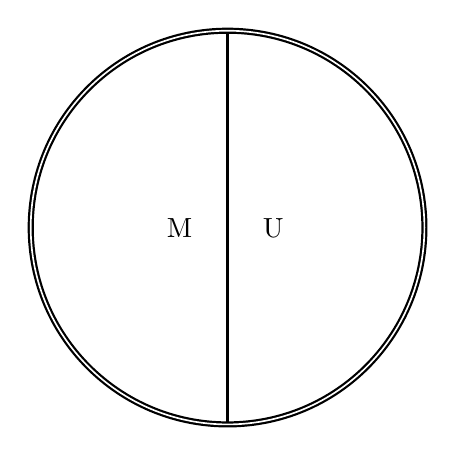
\begin{tikzpicture}[scale=.5]
				\draw[thick,double] (0,0) circle (5);
				\draw[thick] (0,-4.95) -- (0,4.95);
					\node[label={[label distance=2mm]180:M}] at (0,0) {};
					\node[label={[label distance=2mm]360:U}] at (0,0) {};
			\end{tikzpicture}}
		\caption{Syntactic metathesis}\label{fig:SynMet}
  \end{subfigure}
  \begin{subfigure}[b]{0.49\textwidth}
		\centering{\Huge
			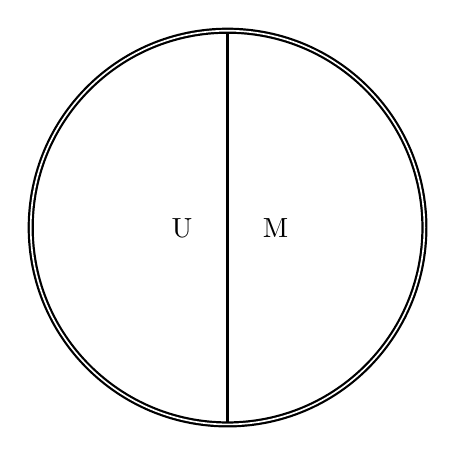
\begin{tikzpicture}[scale=.5]
				\draw[thick,double] (0,0) circle (5);
				\draw[thick] (0,-4.95) -- (0,4.95);
					\node[label={[label distance=2mm]180:U}] at (0,0) {};
					\node[label={[label distance=2mm]360:M}] at (0,0) {};
			\end{tikzpicture}}
		\caption{Discourse metathesis}\label{fig:DisMet}
  \end{subfigure}
	\caption{Complementary metatheses}\label{fig:CompMet}
\end{figure}

An example of each of these complementary pairs
is given below with \qf{ex:120923-2, 1.39 ch:ConCon}
showing a syntactically conditioned M-form‖U-form pair and example
\qf{ex:130909-6, 0.36 ch:ConCon} showing a discourse driven U-form‖M-form pair.

\begin{exe}
	\ex{\glll	na-tuuʔ \bxA{ta\tbr{in}} \bxB{tu\tbr{ni,}} tua, =ma {\lk}\\
						na-tuʔu {\gp}tani {\gp}tuni tua  =ma\\
						\na-make.knot {\gp}rope{\tbrM} {\gp}gewang.palm{\tbrU} {\tua} =and\\
			\glt	`(He) ties up a rope made from gewang palm (leaves)'
						\txrf{120923-2, 1.39} {\emb{120923-2-01-39.mp3}{\spk{}}{\apl}}}\vspace{4pt}\label{ex:120923-2, 1.39 ch:ConCon}
	\ex{\glll	m-ak hai nua =kai \bxA{m-taiko\tbr{bi}} =m hai \bxB{m-ma\tbr{et}} okeʔ {\lk}\\
						m-ak hai nua =kai {\gp}m-taikobi =ma hai {\gp}m-mate okeʔ \\
						\m-say {\hai} two {\kai} \gp\m-fall{\tbrU} =and {\hai} \gp\m-die{\tbrM} all \\
			\glt	`So we two will fall down and (then) both die.'
						\txrf{130909-6, 0.39} {\emb{130909-6-00-39.mp3}{\spk{}}{\apl}}}\label{ex:130909-6, 0.36 ch:ConCon}
\end{exe}

The parallelism and complementarity of U-forms with M-forms
and M-forms with U-forms reflects fundamental Atoni philosophical
and conceptual notions of the structure of the world
as being composed of binary and complementary pairs.
One explicit use of these pairs in linguistic structure is in Amarasi poetry.

\subsection{Metathetic poetic parallelism}\label{sec:MetPoePar}
The role of parallelism in Timor has already been touched on
in \srf{sec:PoePar} in which I discussed the structure of poetry.
Poetry in Amarasi makes use of canonical parallelism \citep{fo88,fo14},
the pairing of pre-determined and semantically related words.
Amarasi poetry is an explicit use of the complementarity
which exists between metathesis and unmetathesis.

Example \qf{ex:140726 0.00--0.05} below,
drawn from a performed chant (\ve{aʔa sramat}) ,
shows the way in which semantic parallelism operates in Amarasi.
Nearly every content word co-occurs in the same line in a structurally
parallel way with a semantically similar content word,
giving three sets of doublets in a single line.
Doublets are joined by linking lines.

\begin{exe}
	\ex{Amarasi chant (\ve{aʔa sramat}): \txrf{140726}{\emb{140726-00-00-00-05.mp3}{\spk{}}{\apl}}}\vspace{5pt}\label{ex:140726 0.00--0.05}
	\begin{xlist}
		\ex{\gll	\bxA{bainesu-t} =ma \bxB{ronaen} n-eu \rnode{C}{\psframebox[linewidth=0.4pt]{mutiʔ}} =ma \rnode{D}{\psframebox[linewidth=0.4pt]{mnatuʔ}} et
							{\lks} {\ncbar[arm=5pt,angle=90,linewidth=0.4pt]{-}{C}{D}}\\
							{\gp}look.up =and {\gp}greeting \n-{\eu} {\gp}silver =and {\gp}gold {\et} \\ \vspace{5pt}}
		\sn{\gll	\bxA{muit} ma-hine-ʔ =ma \bxB{mnatuʔ} neee{\ldots} {\lks}\\
							{\gp}silver {\ma}-know-{\ma} =and {\gp}gold \tsc{pause}\\
				\glt	`Greetings and honour to all people, who are like silver and gold, wise and knowledgeable silver and gold,' \txrf{0.00}}
		\ex{\gll	MA-HINE-Ɂ \\
							{\ma}-know-{\ma} \\
				\glt	`So wise.'	\txrf{0.05}}
	\end{xlist}
\end{exe}

When the doublet consists of a pair of verbs,
it is possible, though not obligatory,
for the first verb to occur in the U-form and the second in the M-form.
Two examples are given in \qf{ex:130825-3, 1.21 ch:ConCon} and \qf{ex:MsimoMaMtoup} below.
In both examples the indicated doublets are both semantically and morphologically parallel.
Thus, for instance, in example \qf{ex:130825-3, 1.21 ch:ConCon}
the semantic doublet, \ve{m-tenu \tcb{‖} mu-haof} `umbrella ‖ shade'
is also a morphological doublet composed of U-form‖M-form.

\begin{exe}
	\ex{\glll	henatiʔ \bxA{m-te\tbr{nu}} =m \bxB{mu-ha\tbr{of}} too tafaʔ =kai {\lks}\\
						henatiʔ {\gp}m-tenu =ma {\gp}mu-hafo too tafaʔ =kai\\
						{\he} \gp\m-umbrella{\tbrU} =and \gp\mu-shade{\tbrM} citizen small {\kai}\\
			\glt	`So that you might shade [doublet] us small people.'
						\txrf{130825-3, 1.21} {\emb{130825-3-01-21.mp3}{\spk{}}{\apl}}}\label{ex:130825-3, 1.21 ch:ConCon}
		\ex{\glll	hai m-nonaʔ =ma m-fee fuaʔturuʔ reʔ hai \\
							hai m-nonaʔ =ma m-fee fuaʔturuʔ reʔ hai \\
							{\hai} {\m}-hand{\Uc} =and {\m}-give offering {\req} {\hai} \\ \vspace{5pt}}\label{ex:MsimoMaMtoup}
		\sn{\glll	\bxA{n-si\tbr{mo}} =ma \bxB{n-to\tbr{up}} =siin mi-ʔko hoo ʔnima-m a-ma-neka-b, {\lks}\\
							{\gp}n-simo =ma {\gp}n-topu =sini mi-ʔko hoo ʔnima-m a-ma-neka-b,\\
							\gp\n-receive{\tbrU} =and \gp\n-receive{\tbrM} ={\siin} {\mi}-{\qko} {\hoo} hand-{\mg} {\at}-{\ma}-love-{\b}\\
							`We give offerings we received from your loving hand.' \txrf{observation}}
\end{exe}

Another kind of metathetic parallelism occurs in chants of the \ve{aʔa sramat} genre.
In such chants a leader of a group will chant one line,
after which the rest of the group repeats a word from that line.
It is common, though not obligatory, for the repeated word 
to occur in the opposite U-form/M-form compared with the form the leader used.
If the leader uses a U-form, the group typically uses an M-form, and vice versa.\footnote{
		Thanks go to Charles Grimes for bringing this to my attention.}

One example is given in \qf{ex:120715-0, 0.30-0.35} below,
in which a verbal U-form said by the leader
is repeated in the M-form by the rest of the group.
Such examples are formally identical to the use of metathesis
in question-answer pairs (\srf{sec:QuePar}).
In each instance one speaker uses a verbal U-form which is completed
by the next speaker(s) using an M-form of the same verb.

\begin{exe}
	\ex{\begin{xlist}
		\ex{\glll	ka= t-tok{\tl}took =ma tak{\tl}t-ak =fa =te, hiit ta-ʔeuk =ma \bxA{\ve{ta-te\tbr{fa}}} =m neee{\ldots}\\
							ka= t-tok{\tl}toko =ma tak{\tl}t-ak =fa =te hiti ta-ʔeku =ma {\gp}ta-tefa =ma neee\\
							{\ka}= \t-{\prd}sit{\M} =and \prd\t-say ={\fa} ={\te} {\hiit} {\ta}-encounter{\M} =and {\gp}{\ta}-meet{\tbrU} =and {\nehh}\\
				\glt	`We don't just sit and talk, we interact and meet.' \txrf{120715-0, 0.30} {\emb{120715-0-00-30-00-35.mp3}{\spk{}}{\apl}}}\
		\ex{\glll \bxA{\ve{TA-TE\tbr{EF}}} \\
							{\gp}ta-tefa \\
							{\gp}{\ta}-meet{\tbrM} \\
				\glt	{\gp}`We meet.' \txrf{0.35}}
	\end{xlist}}\label{ex:120715-0, 0.30-0.35}
\end{exe}

It is also possible for the repeated word to be a noun.
When this occurs, the first instance of the
noun often occurs with a vowel initial enclitic attached
which triggers the M-form (Chapter \ref{ch:PhoMet}).
The whole group will then repeat the noun
without the enclitic; thus in the U-form.
Two examples are given in \qf{ex:140726 1} and \qf{ex:140726 2} below,
each of which comes from a single prayer.

In example \qf{ex:kniunq} the noun phrase \ve{Smana Kninuʔ} `Holy Spirit'
is modified by the determiner \ve{=aa}, and thus occurs in the M-form.
The final word of this noun phrase is then chanted by the whole group, though in the U-form.

\begin{exe}
	\ex{Prayer composed in poetic language: \txrf{140726, 0.21} {\emb{140726-00-21.mp3}{\spk{}}{\apl}}}\label{ex:140726 1}
	\begin{xlist}
		\ex{\glll	iin kuu-n ees reʔ a|n-sia =ma n-naib =kii n-eik ina Smana \bxA{\ve{Kni\tbr{unʔ}=aa}} =m neee{\ldots}\\
							ini kuu-n esa reʔ {\a}n-sia =ma n-nabi =kii n-eki ina smana-f {\gp}kninuʔ=aa =ma neee\\
							{\iin} self-{\N} {\esc} {\req} {\a\n}-lead =ma {\n}-guide{\M} ={\kii} \n-use{\M} {\iin} spirit{\Mc} {\gp}holy{\tbrMv}={\aa} =and {\nehh}\\
				\glt	`It is he who leads and guides us with his Holy Spirit'}\label{ex:kniunq}
		\ex{\gll	RO \bxB{\ve{KNI\tbr{NUɁ}}}\\
							very {\gp}holy{\tbrU}\\
				\glt	`He is very holy.'}\label{ex:kninuq}
	\end{xlist}
\end{exe}

Similarly, in example \qf{ex:areokt} the noun \ve{arekot} `good'
is followed by a vowel initial enclitic and occurs in the M-form.
This word is then repeated by the whole group in \qf{ex:arekot} in the U-form.

\begin{exe}
	\ex{Prayer composed in poetic language: \txrf{140726, 0.27} {\emb{140726-00-27.mp3}{\spk{}}{\apl}}}\label{ex:140726 2}
	\begin{xlist}
		\ex{\glll	etun hii ar=kii m-muiʔ reon =ma runat \bxA{\ve{a-re\tbr{ok}-\tbr{t}=aa}} =m neee{\ldots}\\
							etun hii ar=kii m-muʔi reon =ma runat {\gp}a-reko-t=aa =ma neee\\
							so.that {\hii} all={\kii} \m-have{\M} event =and plan \hspace{1.2mm}\at-good{\tbrMv}-{\at}={\aa} =and {\nehh}\\
				\glt	`So that you will have success in your event and plan.'}\label{ex:areokt}
		\ex{\gll	\bxB{\ve{A-RE\tbr{KO}-\tbr{T}}}\\
							{\gp}{\at}-good{\tbrU}-{\at}\\
				\glt	{\gp}`It is very good.'}\label{ex:arekot}
	\end{xlist}
\end{exe}

The pattern in examples \qf{ex:140726 1} and \qf{ex:140726 2}
with paired nominals is U-form‖M-form, while with verbs
the pattern is M-form‖U-form, as seen in \qf{ex:120715-0, 0.30-0.35}.
The reason noun doublets occur in the order M-form‖U-form,
and verb doublets occur in the order U-form‖M-form
is straightforwardly explained by their order in non-poetic speech.
In the syntax, an M-form noun signals an incomplete attributive
phrase which requires completion from a following form, typically a U-form (Chapter \ref{ch:SynMet}).
In the discourse, a U-form occurs first, and requires resolution
from a subsequent clause, which typically contains an M-form (Chapter \ref{ch:DisMet}).

The use of alternate M-forms and U-forms in Amarasi poetry
-- a style of speech in which parallel forms are obligatory --
is an explicit utilisation of the complementarity which
exists between metathesis and unmetathesis.

\subsection{Cultural and conceptual complementarity}
As discussed in \srf{sec:MetLin}, metathesis is a key
element of the Amarasi language around which many other linguistic structures are organised.
However, more than simply being a key linguistic structure,
the complementarity found between metathesis and unmetathesis
is paralleled by the Atoni conceptualisation of the world
as being composed of complementary parts.

At the beginning of his discussion of the
``Political system as approached in Timorese [Atoni] thinking'',
\citet[408]{scno71} gives a set of complementary concepts,
some of which are given in \trf{tab:AtoParCon}.
Of these concepts he states:
``All these pairs of opposites fit into one scheme and combine to form one important dichotomy.
%All of the concepts in the left-hand column are related by a scheme of mental associations,
%while the same is true of those in the right hand column.
[\ldots] The one is inconceivable without the other.''

\begin{table}[h]
	\caption[Atoni complementary concepts]{Atoni complementary concepts \citep[408]{scno71}}\label{tab:AtoParCon}
	\centering
		\begin{tabular}{rcl} \lsptoprule
			female 		&--& male\\
			wife			&--& husband\\
			sister 		&--& brother\\
			female ancestor	&--&male ancestor\\
			inside		&--&outside\\
			west/north&--&east/south\\
			yellow		&--&red\\
		\lspbottomrule
		\end{tabular}
\end{table}

The Atoni conceptualisation of social and cosmic order
is classified and arranged around such complementary pairs.
A visual analogy of this complementarity can be seen on any piece of Atoni cloth,
illustrated in \frf{fig:AmaSca} below with an Amarasi scarf.
Each half of this cloth, along both horizontal and vertical axes,
is opposite to and a mirror image of the other half;
each half is the complement of the other, and neither is complete without the other.

\begin{figure}[h]\setlength\fboxsep{-0.5pt}\setlength\fboxrule{0.75pt}
	\caption{Amarasi scarf}\label{fig:AmaSca}
	\fbox{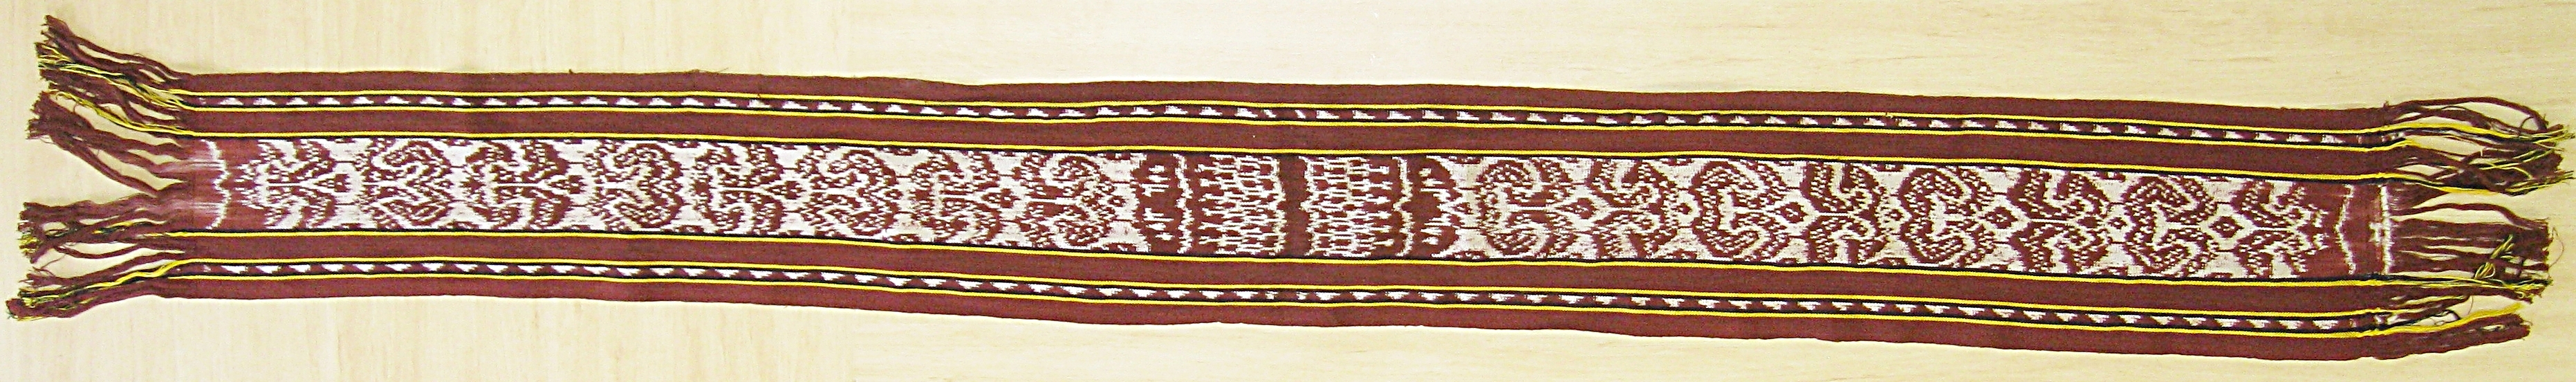
\includegraphics[width=\columnwidth]{AmarasiScarf2.jpg}}
\end{figure}

Dualism and complementarity in the Atoni world
goes beyond the simple ``two-column analysis'' represented in \trf{tab:AtoParCon}.
There are complex relationships between these categories which
include asymmetry, analogical cross-over and recursive parallelism \citep{fo89}.

Of all complementary pairs, one significant relationship
is that of \ve{feto-mone} `female-male'.
A category classified as \ve{feto} `female'
will have a complementary category classified as \ve{mone} `male'.
The classification of pairs as \ve{feto-mone} `female- male'
is not necessarily linked to the actual biological gender
of the members of the pairs,
but is rather a way of expressing and describing
the complementarity which exists between the two categories.

One instance in which the \ve{feto-mone} relationship holds
is in two families related by marriage.
When two families are related by marriage, those who have given their daughter
in marriage (the wife-givers) are classified as \ve{mone} `male'
in relation to those who have received the woman.
Those who have received the woman are classified
as \ve{feto} `female' in relation to the wife givers.

%	Dear Owen
%	No need for confusion. Wife-Giver is Mone; Wife-Taker is Feto.
% As recipient of another’s lineage’s women, that lineage is feto to its wife-giver (mone).
%	Look at my paper (attached) which spells things out explicitly and clearly.
%	Will try to come to your seminar: where will it be? 
%	Will Mark be there?  It would be good to talk to him.
%	Yours, Jim

In addition to being complementary, with each completing the other,
the relationship between the wife-givers and
the wife-receivers is also asymmetrical.
\cite{scno71} analysed this asymmetry in terms of
``superordination'' and ``subordination'':

\begin{quote}
%In the kinship system the \ve{feto-mone} [feminine-masculine] relationship
%is found to exist between two \ve{ume} [houses] which are allied by affinal relationships.
%The \ve{ume} [house] with which the natal \ve{ume} [house] has affinal
%relationships via its daughters is called \ve{feto} [feminine]
%and the one with which it has such relationships via its sons is \ve{mone} [masculine].
``[\ldots] the [female] \ve{ume} [house] receiving a woman (who is the source of life)
is inferior in respect of the [male] one which is the giver of life and hence its superior.
This relationship of subordination and superordination is expressed in terms of \ve{feto-mone}.
But at the same time the term \ve{feto-mone} indicates that the one cannot exist without the other,
as life is impossible without the unity of male and female.
Thus \ve{feto-mone} groups form each other's complements.'' \hfill\citep[411]{scno71}
\end{quote}

While \citeauthor{scno71} accurately identifies the asymmetrical
nature of this relationship the language of ``superordination'' and ``subordination''
may not be the best description of the asymmetry.
Instead, as the givers of the gift, the wife-givers
are in a relationship of precedence to the \ve{feto} `female' wife-receivers \citep{fo94,fo99}.
Because the wife-receivers are \ve{feto} `female' and the wife-givers are \ve{mone} `male',
in this particular context \ve{mone} `male' precedes \ve{feto} `female'.
This is an example of categorical asymmetry \cite[47]{fo94}.

The relationship between \ve{feto} `female' and \ve{mone} `male' groups is not fixed.
As discussed by \cite{fo99}, these relationships are fluid and can be reversed.
Groups constantly seek to re-negotiate their relationship,
with wife-receivers seeking to return a woman to their wife-givers,
and thus reversing their relationship.

A similar conclusion is also reached by \cite{mcw02}
in his study of place and precedence in Amanuban.
While the domain of Amanuban was politically organised with
dual classification, ``these structures tended to
be flexible, strategic, and opportunistic'' \cite[287]{mcw02}.
Complementary categories are tools, not restrictions,
for Atoni thought and classification.

Another area in which the \ve{feto-mone} `female-male'
complementary pair occurs is in the traditional political structure of Atoni society.
In Insana, for instance, the supreme ruler at the centre of a realm
was classified as \ve{feto} `female'.
This \ve{feto} ruler was the guardian of the sacred objects
and responsible for the proper maintenance of ritual.
He was complemented by another ruler, classified as \ve{mone} `male'.
This \ve{mone} ruler was the executive authority of the realm
and had responsibility for warfare \cite[371ff]{scno71}.\footnote{
		Both rulers were biologically male.}

In this context, it would be erroneous to identify
the \ve{mone} `male' ruler as preceding the \ve{feto} `female' ruler.
Instead, it is the supreme \ve{feto} `female' ruler at the centre of the domain,
around whom all the other parts revolve and who holds all these parts together,
who precedes the \ve{mone} `male' ruler.

What is most important in this relationship is the complementarity between
the \ve{feto} `female' ruler and the \ve{mone} `male' ruler,
with both co-existing in balancing roles.
The complementarity between \ve{feto-mone} `female-male',
in which each is one half of a whole,
is represented in \frf{fig:FemMasRel} below.

\begin{figure}
  \begin{subfigure}[b]{0.49\textwidth}
			\centering{\LARGE
				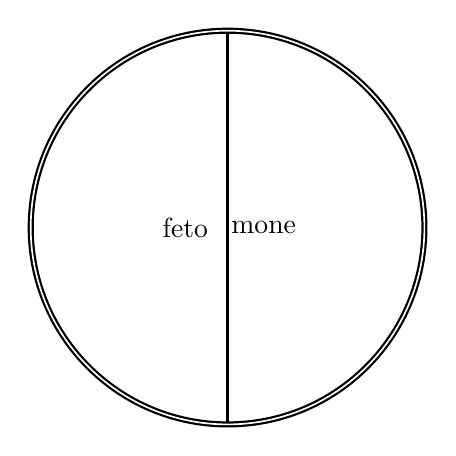
\begin{tikzpicture}[scale=.5]
					\draw[thick,double] (0,0) circle (5);
					\draw[thick] (0,-4.95) -- (0,4.95);
						\node[label={[label distance=-0mm]180:\ve{feto}}] at (0,0) {};
						\node[label={[label distance=-2mm]360:\ve{mone}}] at (0,0) {};
				\end{tikzpicture}}
		\caption{Female-male pair}\label{fig:FemMasRel}
  \end{subfigure}
  \begin{subfigure}[b]{0.49\textwidth}
			\centering{\LARGE
				\begin{tikzpicture}[scale=.5]
					\draw[thick,double] (0,0) circle (5);
					\draw[thick] (0,-4.95) -- (0,4.95);
						\node[label={[label distance=-2mm]180:\ve{moneʔ}}] at (0,0) {};
						\node[label={[label distance=-2mm]360:\ve{nanan\vp{ʔ}}}] at (0,0) {};
				\end{tikzpicture}}
		\caption{Outside-inside pair}\label{fig:OutIns}
  \end{subfigure}
	\caption{Complementary pairs}\label{fig:CompPai}
\end{figure}

Another complementary pair in Atoni thought
is \ve{moneʔ-nanan} `outside-inside', or ``periphery-centre''.
The \ve{nanan} `inside, centre' is symbolic of unity between different parts.
It is the location of the supreme ruler in a realm,
and the area of a house to which agnates
(blood relatives) have full access \citep{cu64}.

Just as the \ve{feto-mone} `female-male' pair is asymmetrical,
the \ve{moneʔ-nanan} `outside-inside' pair is also asymmetrical,
with \ve{nanan} `inside' in precedence to
\ve{moneʔ} `outside' \citep{cu64,scno71,fo89}.
The relationship between the pair \ve{moneʔ-nanan}
is represented in \frf{fig:OutIns}.

The phonological similarity of the terms \ve{mone} `male'
and \ve{moneʔ} `outside' has given rise to a link in Atoni thought
between these two terms and has lead to what \cite{fo89} terms analogical cross-over:
``Male [\ve{mone}], which is superior in certain contexts
is associated with the outside [\ve{moneʔ}], which is inferior'' \cite[49]{fo89}.
The association between \ve{mone} `male' and \ve{moneʔ} `outside',
has also lead to an association between the complements of each of these terms,
with \ve{feto} `female' being associated with \ve{nanan} `inside'.\footnote{
		The term \ve{mone} `male' is a reflex of Proto-Malayo-Polynesian *maRuqanay `male'.
		The term \ve{moneʔ} `outside' is probably
		inherited from Proto-Malayo-Polynesian *ma-udehi `behind',
		also reflected by Amarasi \ve{na-muni} `be at the end' and \ve{munif} `young'.
		Whatever the ultimate etymology of the terms \ve{mone} `male' and \ve{moneʔ} `outside',
		it is the folk etymology ascribed to them by speakers
		which has created (or reinforced) the link between the two \citep[49]{fo89}.}

This association has lead to analogical crossover \citep{fo89}.
The member of each pair with precedence
is linked to the member of the other pair which does not have precedence.
This analogical cross-over is represented in \frf{fig:AnaCro} below
in which each member of each asymmetrical pair is connected
with the opposite member of the other asymmetrical pair.

\begin{figure}[h]
\caption{Analogical cross-over}\label{fig:AnaCro}
	\begin{minipage}{.49\textwidth}
			\centering{\LARGE
				\begin{tikzpicture}[scale=.5]
					\draw[thick,double] (0,0) circle (6);
					\draw[thick,double] (-5.95,0) -- (5.95,0);
					\draw[thick] (0,-5.95) -- (0,5.95);
						\node(a)[label={[label distance=-7mm]90:\ve{feto}}] at (-2.5,2.5) {};
						\node(b)[label={[label distance=-5mm]90:\ve{mone}}] at (2.5,2.5) {};
						\node(c)[label={[label distance=-8mm]90:\ve{moneʔ}}] at (-2.5,-2.5) {};
						\node(d)[label={[label distance=-8mm]90:\ve{nanan}}] at (2.5,-2.5) {};
						\draw[thick,<->] (a) -- (d);
						\draw[thick,<->] (c) -- (b);
				\end{tikzpicture}}
	\end{minipage}
	\begin{minipage}{.49\textwidth}
			\centering{\LARGE
				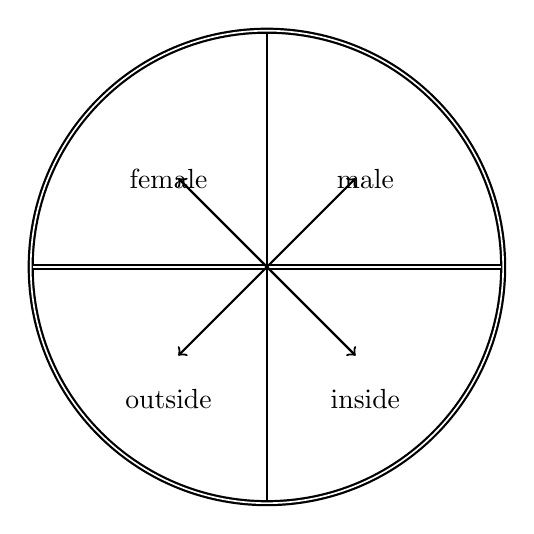
\begin{tikzpicture}[scale=.5]
					\draw[thick,double] (0,0) circle (6);
					\draw[thick,double] (-5.95,0) -- (5.95,0);
					\draw[thick] (0,-5.95) -- (0,5.95);
						\node(a)[label={[label distance=-5mm]90:{female}}] at (-2.5,2.5) {};
						\node(b)[label={[label distance=-5mm]90:{male}}] at (2.5,2.5) {};
						\node(c)[label={[label distance=-8mm]90:{outside}}] at (-2.5,-2.5) {};
						\node(d)[label={[label distance=-8mm]90:{inside}}] at (2.5,-2.5) {};
						\draw[thick,<->] (a) -- (d);
						\draw[thick,<->] (c) -- (b);
				\end{tikzpicture}}
	\end{minipage}
\end{figure}

One instance of this association has been seen in the fact that the \ve{feto} `female ruler
is located in the \ve{nanan} `centre' of the realm.
Another example of this association in Amarasi is seen in the categorisation
of the \ve{tasi} `sea, ocean', which is classified as consisting of two parts.
The \ve{nanan} `inner' circle of sea near the coast and bays
is the \ve{tais feto} `female sea', and the distant \ve{moneʔ} `outer' part
is known as the \ve{tais mone} `male sea' \cite[50]{cu64}.
This means that the northern Savu Sea is the \ve{tais feto} `female sea'
and the southern Timor Sea is the \ve{tais mone} `male sea',
as illustrated in \frf{fig:TimSea}

\begin{figure}[h]
	\caption{Timor and its seas}\label{fig:TimSea}
	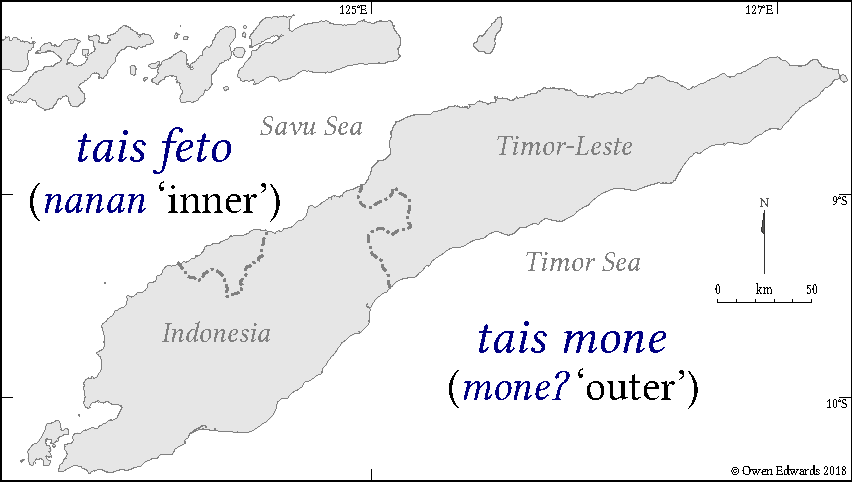
\includegraphics[width=0.8\columnwidth]{TimorSeas.pdf}
\end{figure}

\subsection{Metathetic parallel complementarity}\label{sec:MetParCom}
It is within this rich world of symbolic dualistic and complementary
classification that I place my analysis of metathesis in Amarasi.
Unmetathesised forms and metathesised forms are one another's complements.
This is demonstrably a fact of linguistic structure.
In the syntax, an M-form cannot occur in isolation and must be completed by a U-form.
In the discourse a U-form does not occur alone
and must be completed by another form, typically an M-form.

The identification of U-forms and M-forms as complementary pairs
is not equivalent to noting that these forms are formal opposites.
Instead, this identification is based on their usage,
the fact that each form must occur with the other in certain contexts.
Furthermore, in Amarasi poetry
-- a genre in which parallelism is obligatory --
unmetathesised and metathesised forms
are explicitly used as complementary pairs,
as discussed in \srf{sec:MetPoePar} above. %\footnote{
		%That U-forms and M-forms are complementary pairs
		%and not merely opposites can be illustrated with a negative example.
		%Within Amarasi phonology the phoneme /b/
		%and the phoneme /p/ are opposites:
		%/b/ is a voiced obstruent and /p/ is a voiceless obstruent.
		%However, there is no instance in which these two phonemes are deliberately paired together.
		%These two phonemes may be opposites, but they are not complements.}

Syntactic M-forms (M\sub{\tsc{s}}) are complemented and completed by syntactic U-forms (U\sub{\tsc{S}}),
and discourse U-forms (U\sub{\tsc{d}}) are completed and complemented by discourse M-forms (M\sub{\tsc{d}}).
In addition, the syntactic M\sub{\tsc{s}}‖U\sub{\tsc{s}} relationship
is itself paralleled and complemented by the opposite discourse U\sub{\tsc{d}}‖M\sub{\tsc{d}} relationship.
That M-forms require completion in the syntax is paralleled by the fact
that in the discourse it is U-forms which require completion.
The parallel relationship between the syntactic M\sub{\tsc{s}}‖U\sub{\tsc{s}} pair
and discourse U\sub{\tsc{d}}‖M\sub{\tsc{d}} pairs is represented in \frf{fig:AmaMet} below.
With an example of each given in \qf{ex:120923-2, 1.39 ch:ConCon2} and \qf{ex:130909-6, 0.36 ch:ConCon2}.

\begin{figure}[h]
	\caption{Metathesis and unmetathesis in Amarasi}\label{fig:AmaMet}
	\centering{\Huge
		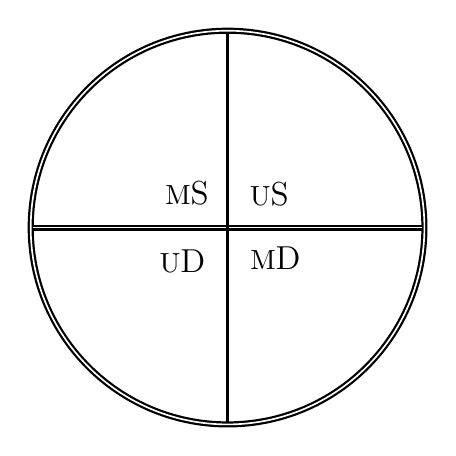
\begin{tikzpicture}[scale=.5]
			\draw[thick,double] (0,0) circle (5);
			\draw[thick,double] (-4.95,0) -- (4.95,0);
			\draw[thick] (0,-4.95) -- (0,4.95);
				\node[label={[label distance=.5mm]45:U\sub{\large S}}] at (0,0) {};
				\node[label={[label distance=.5mm]125:M\sub{\large S}}] at (0,0) {};
				\node[label={[label distance=.5mm]325:M\sub{\large D}}] at (0,0) {};
				\node[label={[label distance=.5mm]225:U\sub{\large D}}] at (0,0) {};
		\end{tikzpicture}}
\end{figure}

\begin{exe}
	\ex{Syntactic metathetic complementarity M\sub{\tsc{s}}‖U\sub{\tsc{s}}:}\vspace{4pt}\label{ex:120923-2, 1.39 ch:ConCon2}
	\sn{\glll	na-tuuʔ \bxA{ta\tbr{in}} \bxB{tu\tbr{ni,}} tua, =ma {\lk}\\
						na-tuʔu {\gp}tani {\gp}tuni tua  =ma\\
						\na-make.knot {\gp}rope{\tbrM\tbr{\sub{\tsc{s}}}} {\gp}gewang.palm{\tbrU\tbr{\sub{\tsc{s}}}} {\tua} =and\\
			\glt	`(He) ties up a rope made from gewang palm (leaves)'
						\txrf{120923-2, 1.39} {\emb{120923-2-01-39.mp3}{\spk{}}{\apl}}}\vspace{4pt}\label{120923-2, 1.39 ch:ConCon}
	\ex{Discourse metathetic complementarity U\sub{\tsc{d}}‖M\sub{\tsc{d}}:}\vspace{4pt}\label{ex:130909-6, 0.36 ch:ConCon2}
	\sn{\glll	m-ak hai nua =kai \bxA{m-taiko\tbr{bi}} =m hai \bxB{m-ma\tbr{et}} okeʔ {\lk}\\
						m-ak hai nua =kai {\gp}m-taikobi =ma hai {\gp}m-mate okeʔ \\
						\m-say {\hai} two {\kai} \gp\m-fall{\tbrU\tbr{\sub{\tsc{d}}}} =and {\hai} \gp\m-die{\tbrM\tbr{\sub{\tsc{d}}}} all \\
			\glt	`So we two will fall down and (then) both die.'
						\txrf{130909-6, 0.39} {\emb{130909-6-00-39.mp3}{\spk{}}{\apl}}}
\end{exe}

This is an example of analogical cross-over similar to
the association between \ve{feto-mone} `female-male'
and \ve{moneʔ-nanan} `outside-inside' discussed above.
In the case of metathesis, the association
is not between two formally similar (and perhaps related) forms
but instead it is between two formally identical forms,
with the same derivation which occur at different levels of the grammar.

The relationship between the four metathesis forms in \frf{fig:AmaMet} is
an instance of what I term ``cyclical complementarity''.
A syntactic M-form is complemented by a syntactic U-form,
which is paralleled by a discourse M-form which is the complement
of a discourse U-form, which is paralleled by a syntactic M-form,
and so on \emph{ad infinitum}.
Such cyclical complementarity is also found in
systems of marriage exchange in this region (whether formalised or informal),
whereby the wife-receivers will eventually return a woman to their wife-givers,
and thereby become the wife-givers, and so on.
Among the Atoni, for instance:

\begin{quote}
``[\ldots] it is to the advantage of wife-givers to maintain their
asymmetric relation with their wife-takers and to the advantage of wife-takers
to reverse this relationship by returning a woman to their wife-givers [\ldots]''
\cite{fo99}
%\hfill \cite[32]{fo99}
\end{quote}

The complementarity between metathesis and unmetathesis in Amarasi
and its strong congruence with the conceptual framework,
cosmic classification and social organisation of Amarasi speakers
raises a number of interesting questions,
which I only pose up at this point.

Firstly, to what extent does the complementarity between unmetathesis and
metathesis occur in other Meto varieties?
Speakers of other Meto varieties have the same conceptual frameworks
as speakers of Amarasi. Thus, we expect this relationship to hold,
even if U-forms and M-forms have different forms and functions.
To answer this question will require a detailed study of
metatheses across other varieties of Meto.

Secondly, is the prevalence of synchronic metathesis in the greater Timor region
(see \frf{fig:CVMetTimReg} on page \pageref{fig:CVMetTimReg}) linked in any way
to the widespread use of complementary and dualistic classification in this region?
To answer this question will require a study of whether other regions
in which complementarity is common also have linguistic structures
which are complementary in a way that parallels that of metathesis in Amarasi.

Finally, how did the complementary nature of metathesis and unmetathesis arise in Amarasi?
Is it simply an accidental by-product of the environments
in which a phonological process became morphological?
Or is it a result of speakers (consciously or unconsciously)
noticing things about culture and mirroring them in grammar, and vice versa?
%If the latter, this could indicate that the any grammar-culture barrier
%is considerably more porous than some have thought.

One fruitful avenue of work which may help answer this last
question is a thorough structural examination of poetry and
verbal art in Meto. In poetry the complementarity of U-forms
and M-forms is explicitly utilised by speakers in more fluid
way than is seen in the syntax or discourse.
It may be the case that poetry was the domain of
language in which the complementarity between U-forms and M-forms first began.

For now, however, the last word and final statement on the
source and origin, as well as the reasons and grounds
of the parallelism and complementarity of metathesis and unmetathesis
in Amarasi should be given to the Amarasi speakers themselves,
expressed in their own poetic language composed in parallel pairs:

\begin{exe}
	\ex{Chant (\ve{aʔa sramat}) performed at a wedding service:
			\txrf{090524, 0.36} {\emb{090524-00-36.mp3}{\spk{}}{\apl}}}\vspace{4pt}\label{ex:24/05/2009}
	\begin{xlist}
		\ex{\glll	ar=kiit \bxA{ta-hiin} =ma \bxB{ta-keo} moni-t mansian {\lks}\\
							ar=kiti \gp{ta-hini} =ma \gp{ta-keo} moni-t mansian \\
							all={\kiit} \gp\ta-know{\M} =ma \gp\ta-aware live{\U}-{\at} human\\}\vspace{4pt}
		\sn{\glll	pasan{\tl}pasan, \bxA{bifee} \bxB{atoniʔ\vp{f}}
							\rnode{C}{\psframebox[linewidth=0.4pt]{feto-f}}
							\rnode{D}{\psframebox[linewidth=0.4pt]{nao-f}}
							{\lks}{\ncbar[arm=5pt,angle=90,linewidth=0.4pt]{-}{C}{D}}\\
							pasan{\tl}pasan {\gp}bifee {\gp}atoniʔ {\gp}feto-f {\gp}nao-f \\
							{\frd}pair {\gp}woman {\gp}man {\gp}sister-{\F} {\gp}brother-{\F}\\}\vspace{4pt}
		\sn{\glll \bxA{ta-bua} \bxB{ta-ʔ-mees-ʔ=oo-k} n-bi {\lks}\\
							\gp{ta-bua} \gp{ta-ʔ-mese-ʔ=oo-k} n-bi\\
							\gp\ta-gather {\gp\ta-\qV-one{\Mv}-\qV=\oo-\k} {\n-\bi}\\}\vspace{4pt}
		\sn{\gll \bxA{bare} a-reko-t \bxB{paha} =t neee,{\ldots} {\lks}\\
							{\gp}place {\at-good-\at} {\gp}country ={\te} {\nehh}\\
				\glt	`We all know and are aware that the life of humans comes in pairs;
							woman and man, sister and brother, gathered together in unity,
							in places and countries that are good.'}
		\ex{\gll	\ve{RO REKO} {}\\
							{`It is very good.'} {} \\}
	\end{xlist}
\end{exe}
